\documentclass[onecolumn, 12pt, a4paper]{article}
\usepackage[margin=1.00in]{geometry}
\usepackage{natbib}
\bibliographystyle{icarus}
\usepackage{amsmath}
\usepackage{amssymb}
\usepackage{subcaption}
\usepackage{graphicx}
\usepackage{caption2}
\usepackage{tabu}
\usepackage{multirow}
\begin{document}



\providecommand{\e}[1]{\ensuremath{\times 10^{#1}}}

\setlength{\parskip}{0em}


\onecolumn{%}
 \centering
 \LARGE Lab #2 Report: Astronomical Spectroscopy: Detecting Light With A CCD \\[1.5em]
 %\LARGE Deformation of Mars shorelines explained by Tharsis uplift and limited true polar wander \\[1.5em]
 \large Eden Chen,
        Magdelena Allen, 
        and Joseph Miller

 October 10, 2017
 
 Email: ychen3856@berkeley.edu \linebreak
 Student ID: 3032340806

\vspace{0.25in}

}

    
%\title{Building the Moon from Multiple Impacts: Merger Efficiency and Dynamical Constraints}
%\author{Robert I. Citron$^{1}$, Hagai B. Perets$^{2}$, and Oded Aharonson$^{3}$}
%\affil{$^{1}$Department of Earth and Planetary Science, University of California Berkeley, Berkeley, California, USA}
%\affil{$^{2}$Department of Astrophysics, Israel Institute of Technology, Haifa, Israel}
%\affil{$^{3}$Department of Earth and Planetary Science, Weizmann Institute of Science, Rehovot, Israel}


\begin{abstract}
In this experiment we used an Ocean Optics USB 2000 Spectrometer to collect various light spectra samples ranging from fluorescent light, neon light to incandescent light. By examining the emission and absorption lines in the spectra we can determine what elements are present in a certain light source. Since each emission line's peak positions in wavelength and pixel number will not be the exact position of the elemental signature like Mercury (Hg I) and Neon (Ne I) emission lines, we will need to find the center of mass for each emission line, that is the centroid, and use the method of linear least squares to determine a polynomial fit. However the linear least squares method did not work well with the combined Hg I and Ne I centroid plot, so we used a second degree polynomial method to create a quadratic fit line and determine its error. We can then calculate the read noise and the gain of the CCD detector. We calculated the gain to be 0.6307846 and read noise to be 5.4503907. The standard deviation of the gain is $7.0005e{-3}$ and 0.003151 for the read noise. We also measured the saturation level of the CCD detector to be 4096 counts.
\end{abstract}

\section{Introduction}  \label{introduction}

By using a spectrometer we can examine emission lines and absorption lines created by different elements in the light emitted from a specific source. Incandescent lamp, fluorescent strip light, color filters, neon gas discharge lamp, and sunlight all presents a unique spectra of light based on the emission and absorption lines. Emission lines occurs when an atom, element or molecule in an excited state loses energy and transition to a lower energy state. Since each atom, element and molecule all possess a unique set of energy levels they will emit photons at different wavelength and produces energy equal to the difference between the initial and final state. Absorption lines occur when there exist an opaque material like a cloud of gas or a piece of filter in between the spectrometer and the source. Different atom, element and molecule present in that material can absorb energies at a different set of wavelength thus create dark spots in the spectra which we called absorption lines. We will be determining the wavelength calibration of the spectrometer. We do it by mapping the centroids of each fluorescent and neon emission line between pixel number and wavelength. Furthermore, we will use the method of linear least square to fit a line for both fluorescent and neon centroid plots and compare them both to test the reliability of the method by specifying the errors in the slope and intercept. Finally, we will measure the gain, read noise and the saturation level of the CCD Photon Detector.

\section{Methods} \label{methods}
All plots and results in this experiment are achieved using the Python coding software. In this experiment we used two methods: equation to find the centroid and the linear least squares. We find the centroids $<x>$ of each emission lines using: 

\[<x> = \sum_{i}{X_i I_i }/{I_i}\]  

To find multiple centroids in a set of data with different bumps that represents emission lines we will need to use the Full Width at Half Maximum method (FWHM).  FWHM is a parameter commonly used to describe the width of a bump on a curve or function. It is given by the distance between points on the curve at which the function reaches half its maximum value. We will also be using the method of linear least squares to fit a line to each sets of data and determine their standard deviations. The equation of a straight line would just be: 

\[y = mx + c\] 

where y is the intensity, m as the slope, c is the initial position and x can be the wavelength or pixel number. For the read noise and gain of the CCD detector we will be using:

\[\sigma^2_{ADU} = \frac{g \times e}{C} \times (ADU - ADU_o) + \sigma^2_{o}\]

where $\frac{g \times e}{C}$ is the gain and $\sigma^2_{o}$ is the read noise. Notice how it can be related to y = mx + c where the gain is the slope m and the read noise is the y-intercept c. 

\section{Equipment} \label{Equipment}
The experiment setup consists of an Ocean Optics USB 2000 Spectrometer with a compatible program called SpectraSuite. The USB 2000 is an optical spectrometer that uses a diffraction grating and a one-dimensional CCD detector array. The CCD array is made up of 2048 pixels in a linear array, so the spectrum reads out as a list of 2048 pixel numbers. The spectrometer can be connected to a optical fiber with a SMA 905 plug to make the setup more flexible. This spectrometer has a spectral resolution of about 0.6 nanometer (nm) with the wavelength range of 370 to 700 nm. 

\section{Acquiring Data} \label{acquiring_data}
On September 26, 2017, Joe, Elena and I collected our first sets of data with the spectrometer located at Campbell Hall, University of California Berkeley. We collected spectra from various light sources including incandescent lamp, fluorescent strip light, color filters, neon gas discharge lamp, and sunlight. All the above data sets were have 100 integration time and collected in pair: one in wavelength and one in pixel number. We have also collected one set of dark current by covering the slit completely. Unfortunately the spectrometer and the optical fiber malfunctioned on October 6, 2017 so my group and I had to collect additional sets of data by accessing the archived data from the previous semester.

\section{Data Processing} \label{data_proccessing}
By plotting various spectra data collected from the spectrometer we can see different light sources will produce different sets of emission line. \newline

  \begin{subfigure}{\linewidth}
  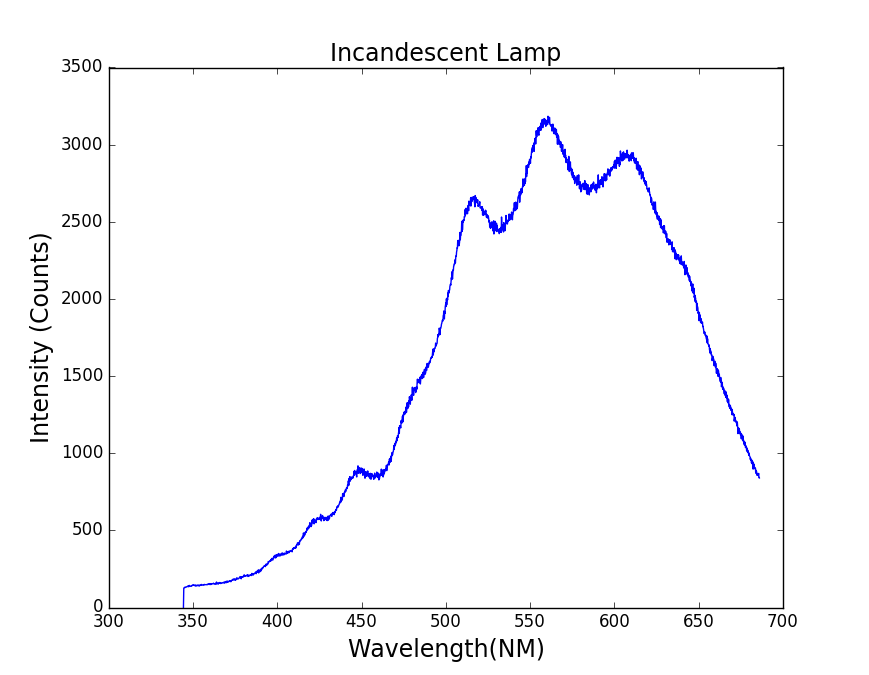
\includegraphics[width=.5\linewidth]{Incan.png}
  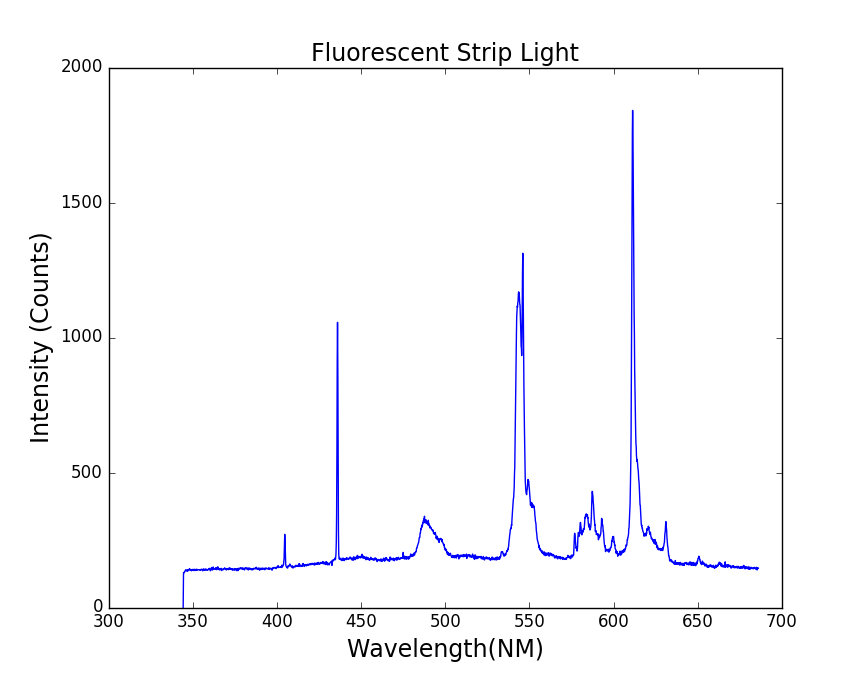
\includegraphics[width=.5\linewidth]{Fluor.png}
  \end{subfigure}\par\medskip
  \begin{subfigure}{\linewidth}
  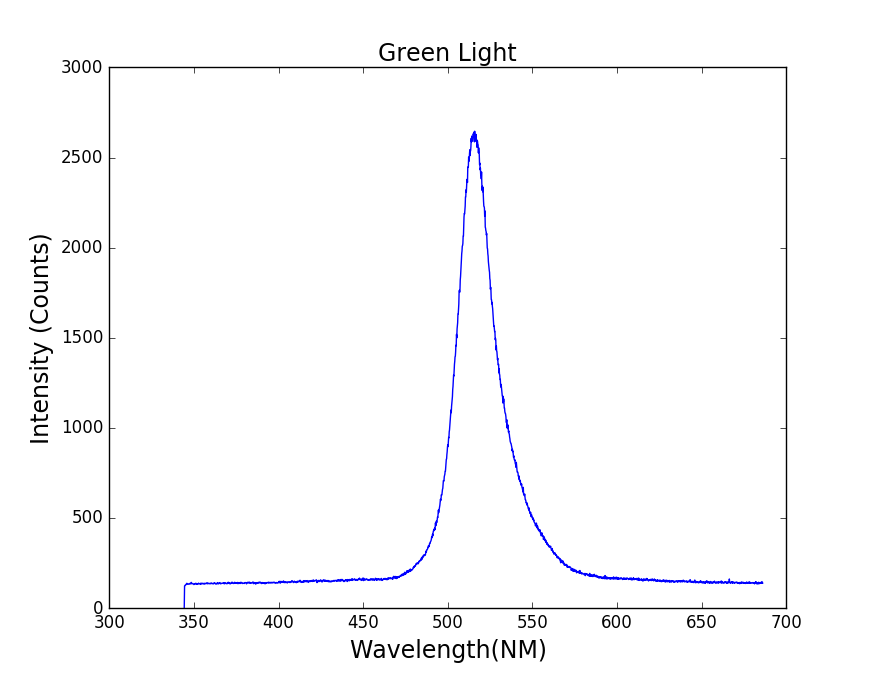
\includegraphics[width=.5\linewidth]{Greenlight.png}
  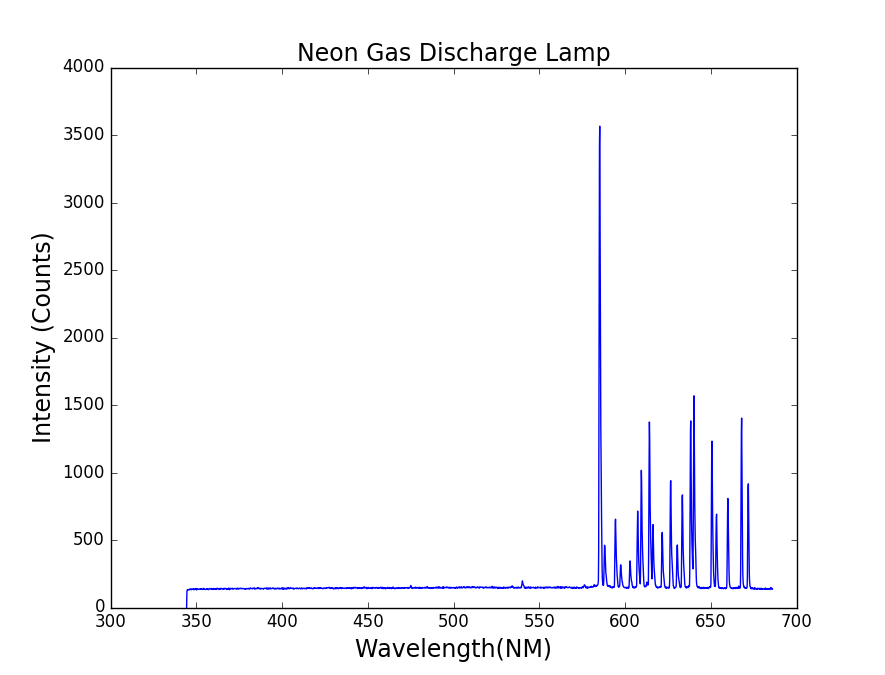
\includegraphics[width=.5\linewidth]{neon.png}
  \centerline{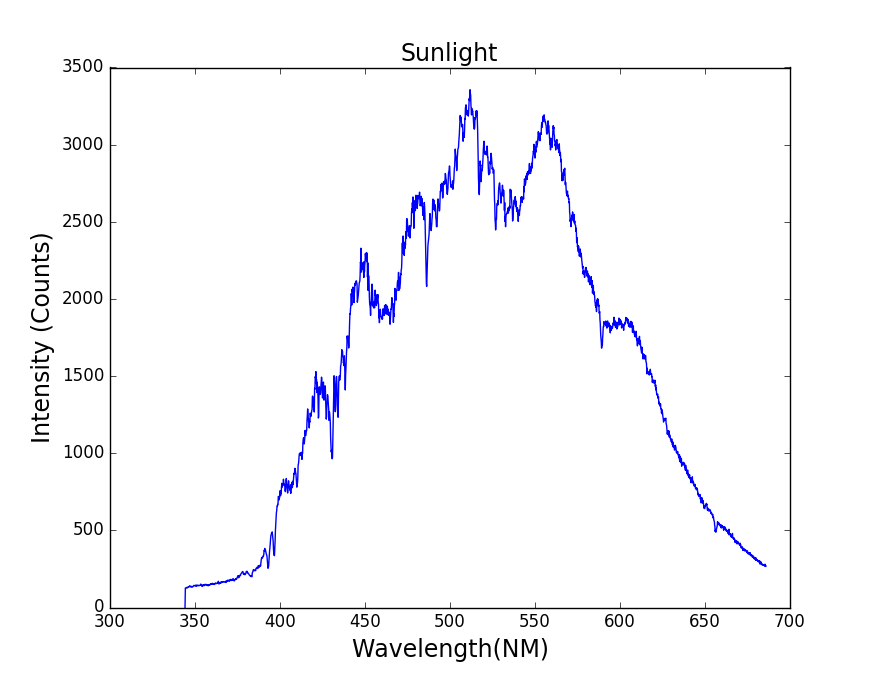
\includegraphics[scale=.4]{sunlight.png}}
  \end{subfigure}\par\medskip
  \linebreak
  Figure 1: Spectra of various light sources in wavelength with integration time of 100 milliseconds (ms). For the mapping of centroids between pixel number and wavelength we will only be using fluorescent strip light and neon gas discharge lamp. Notice how each plots have elevated overall intensity of roughly 120 counts. That is because these plots are not calibrated by subtracting out the bias.


\newpage

Here is a plot of the bias spectra, achieved by covering up the spectrometer slit and collect the data:

\hspace*{-1cm}\centerline{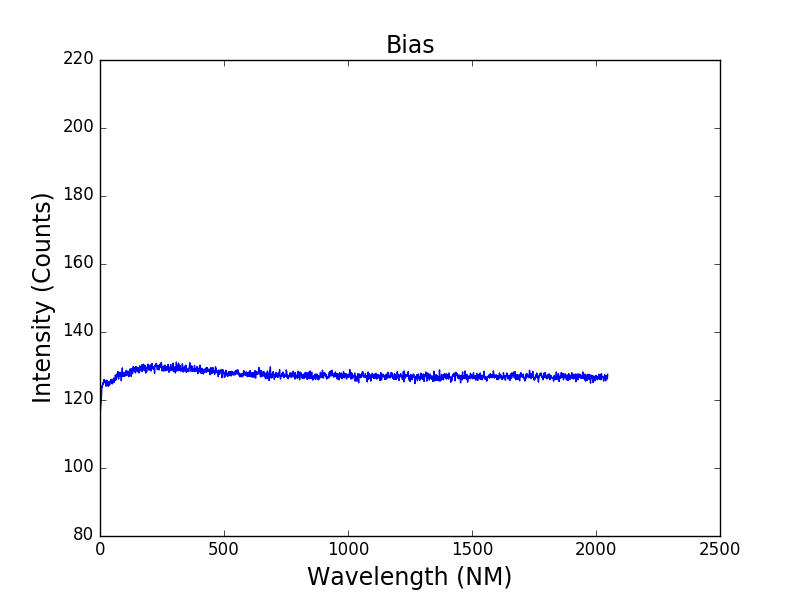
\includegraphics[scale = .35]{bias.png}}

\centerline{Figure 2: The bias spectra collected with the integration time set to 3ms.} 

\begin{flushleft}
By subtracting the fluorescent light and neon light spectra with the bias spectra we can create a bias subtracted graph for both spectra:
\end{flushleft}

  \begin{subfigure}{\linewidth}
  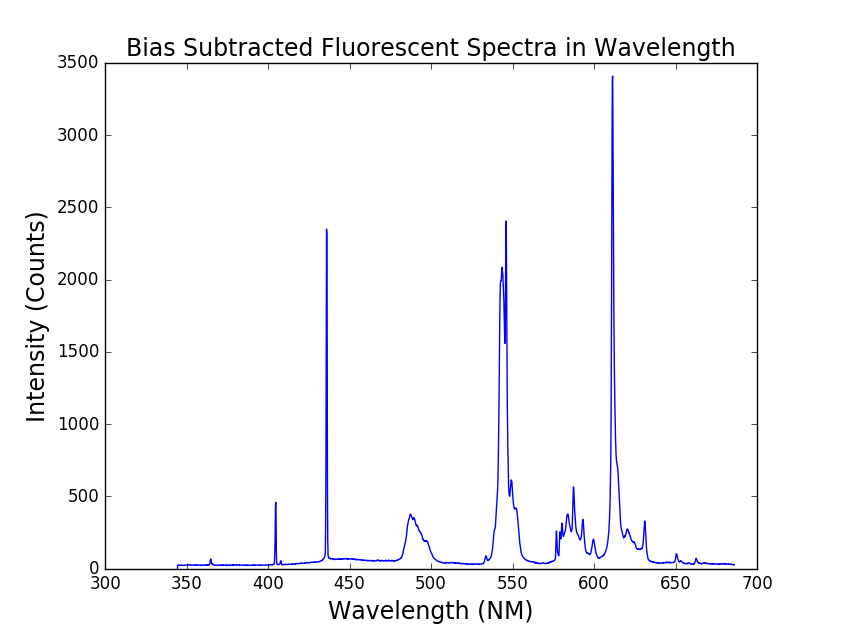
\includegraphics[width=.44\linewidth]{biasfluor.png}
  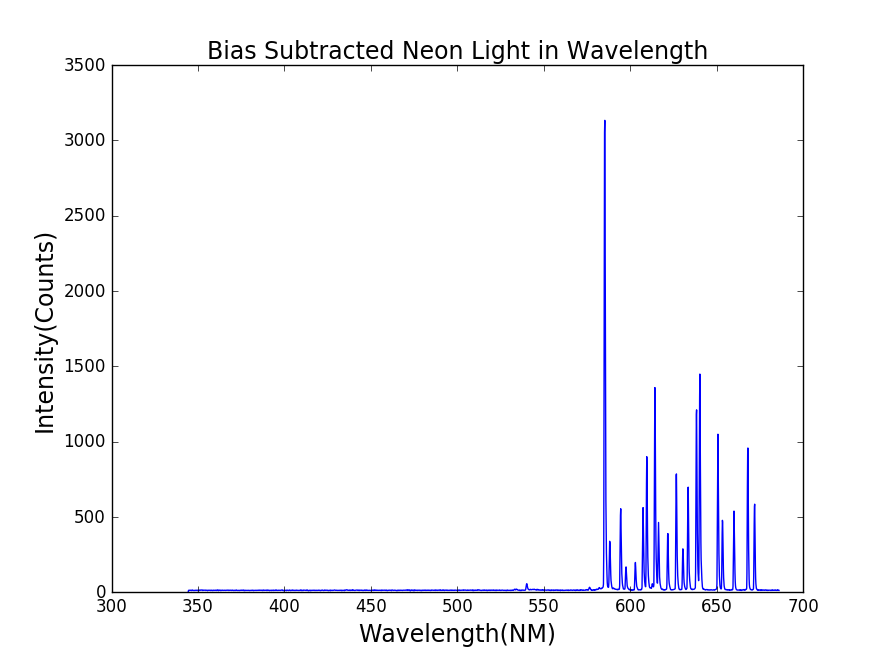
\includegraphics[width=.45\linewidth]{biasneon.png}
  \end{subfigure}\par\medskip
  \begin{subfigure}{\linewidth}
  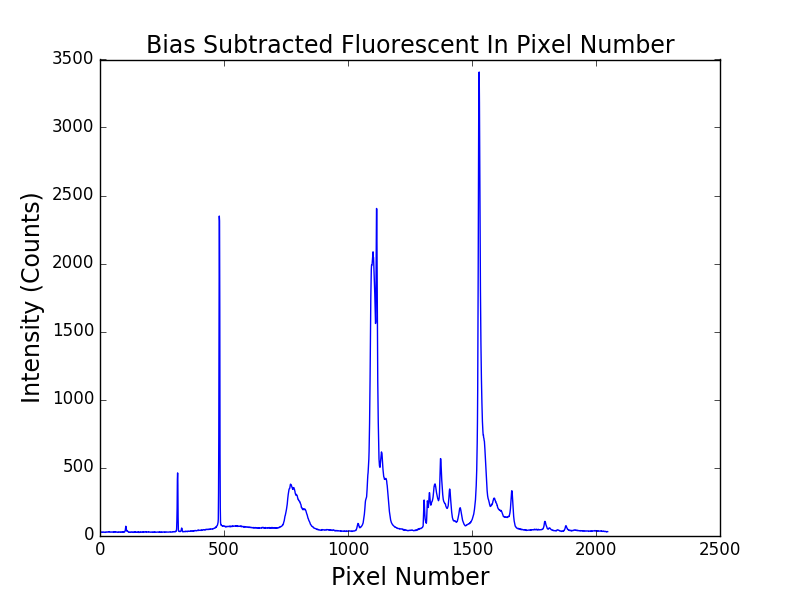
\includegraphics[width=.45\linewidth]{pbiasfluor.png}
  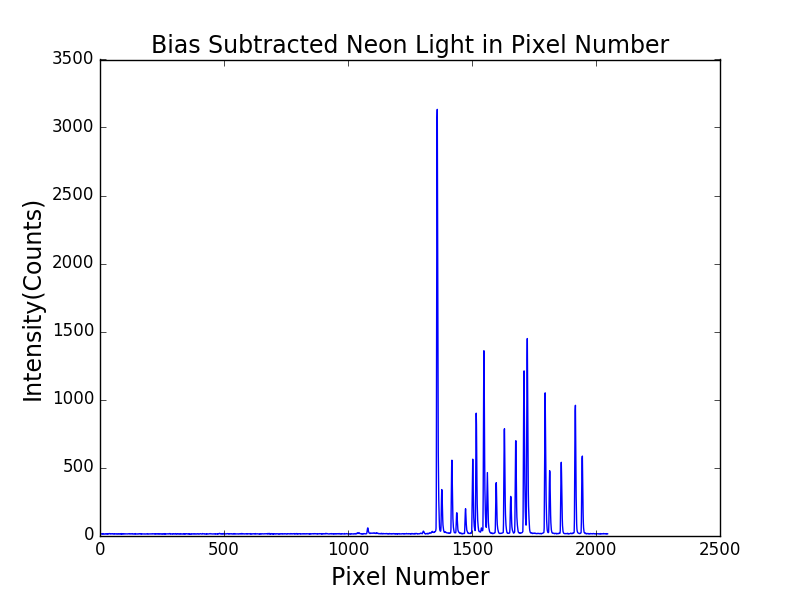
\includegraphics[width=.45\linewidth]{pbiasneon.png}
  \end{subfigure}\par\medskip
  \newline 
\begin{flushleft}
Figure 3: The bias subtracted plot of fluorescent and neon spectra in wavelength and pixel number. As we can see that the overall intensity for all four plots have decreased by the amount equal to the average intensity of the bias spectra.
\end{flushleft}
\newline
\section{Wavelength Calibration} \label{calibration}
In order to measure the read noise and gain of the CCD detector we first need to determine the wavelength calibration of the spectrometer by mapping the centroid of Hg I and Ne I emission lines in pixel number and wavelength. We can then fit a linear line for the centroids of both element separately and measure the standard deviations of their slope and y-intercept. To further calibrate our wavelength we will combine the centroids from both element and show that the linear fit line do not work well with higher degree polynomials.

\subsection{Centroids} \label{centroids}
Although we can visually identify the position of each peaks, they do not represent the exact location of the emission lines for a specific element. We can find the true position by measuring the Centroid of each emission lines using 

\[<x> = \sum_{i}{X_i I_i }/{I_i}\].

Where $I_i$ is our intensity and $X_i$ can be our wavelength or pixel number. By using the FWHM method we can use Python to repeatedly determine a range of wavelength or pixel number at different peaks and use it to plug into our centroid equation. Combing the centroid equation and FWHM to the bias subtracted fluroescent and neon spectra in both wavelength and pixel number gives us:

\begin{subfigure}{\linewidth}\hspace*{-1.2cm}
  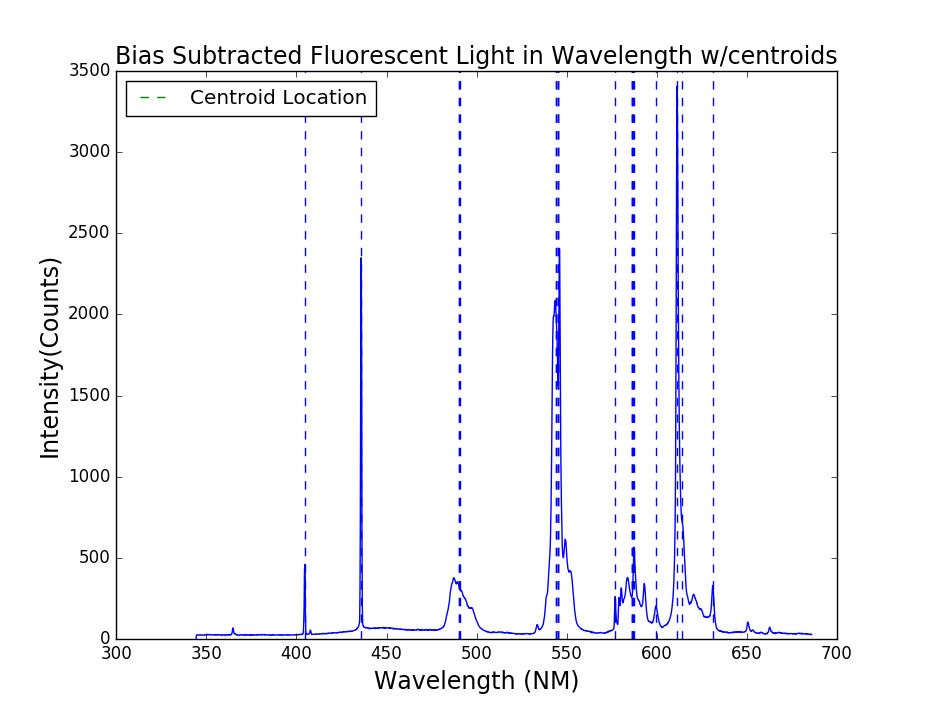
\includegraphics[width=.55\linewidth]{fcentw.png}
  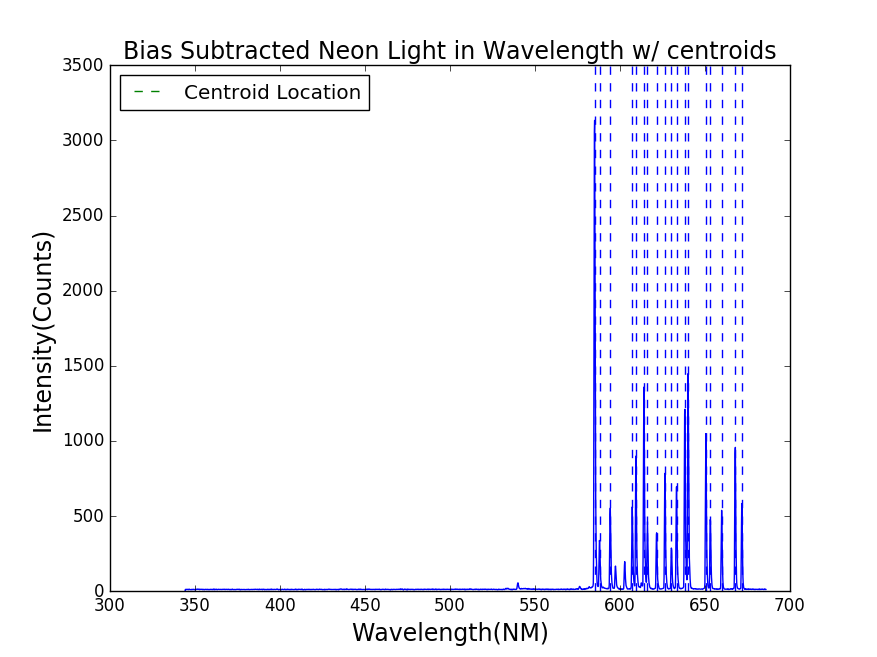
\includegraphics[width=.55\linewidth]{neoncentw.png}
  \end{subfigure}\par\medskip
  \begin{subfigure}{\linewidth}\hspace*{-1.2cm}
  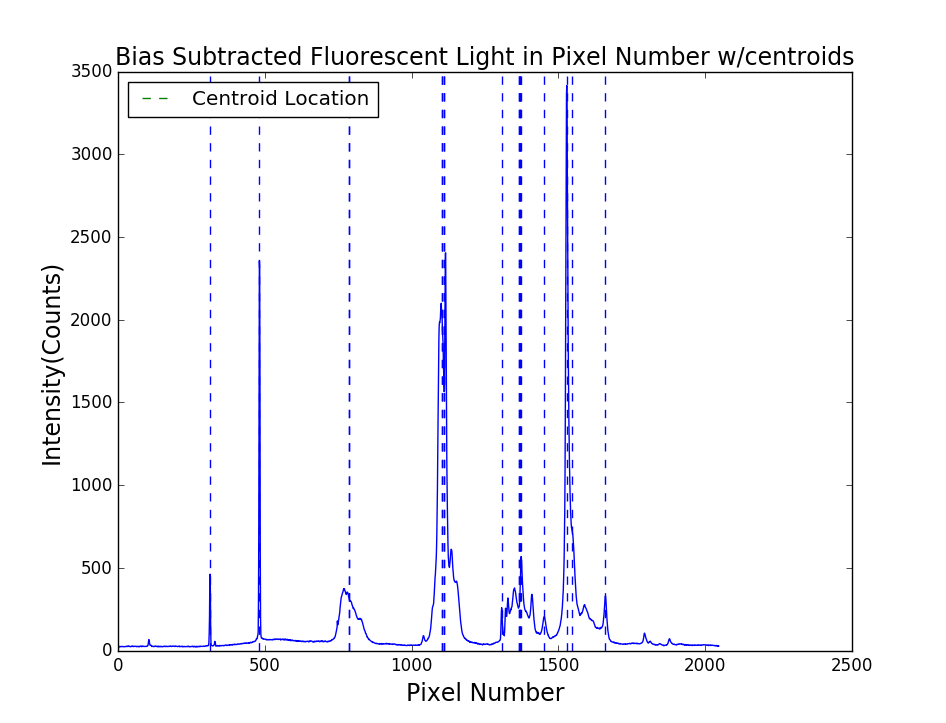
\includegraphics[width=.55\linewidth]{fcentp.png}
  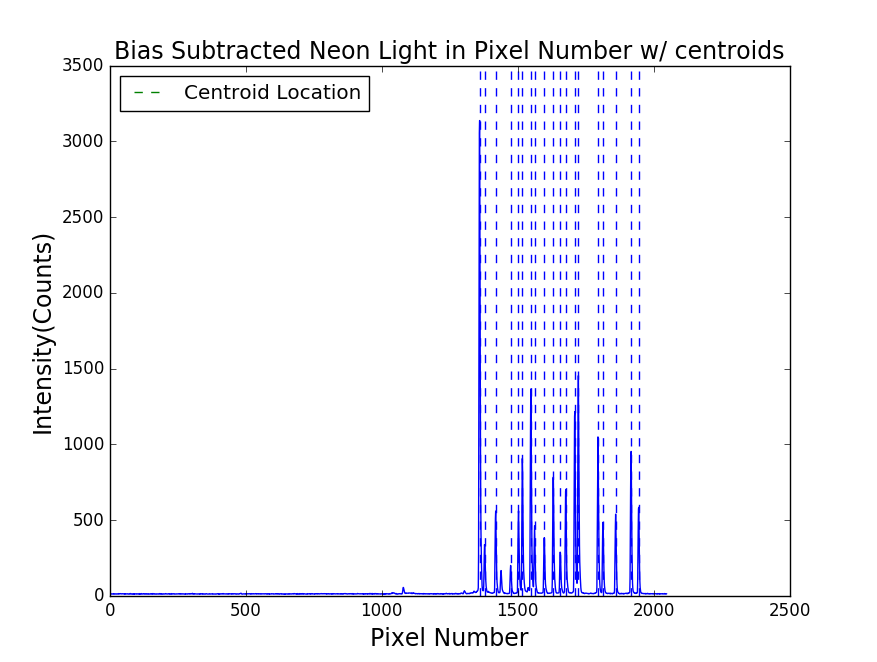
\includegraphics[width=.55\linewidth]{neoncentp.png}
  \end{subfigure}\par\medskip
  \newline
\begin{flushleft}
Figure 4: Same graphs as Figure 3 but with centroid locations listed with dash lines. If examine closely, we can see that each centroid does not have the same wavelength or pixel number as the peaks. These centroids can tell us the true location of a specific element's emission lines.
\end{flushleft}
\newline
In this experiment we only want to identify the location of Hg I emission lines in the fluorescent light and Neon Ne I emission lines in the neon light. I extracted total of seven Hg I lines from the fluorescent light and ten Ne I emission lines from the neon light. We should expect a linear behavior by comparing the extracted centroids in wavelength against pixel number.

\begin{subfigure}{\linewidth}\hspace*{-1.3cm}
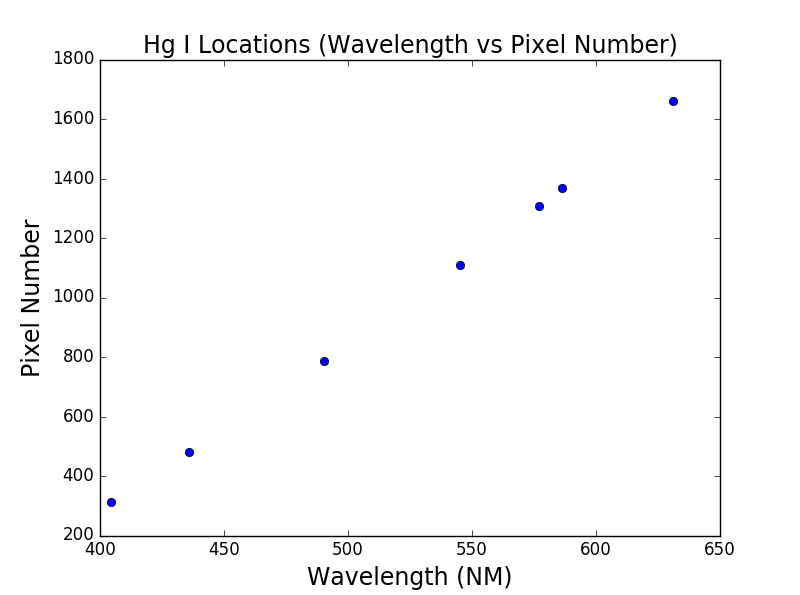
\includegraphics[width=.55\linewidth]{Hg1loc.png}
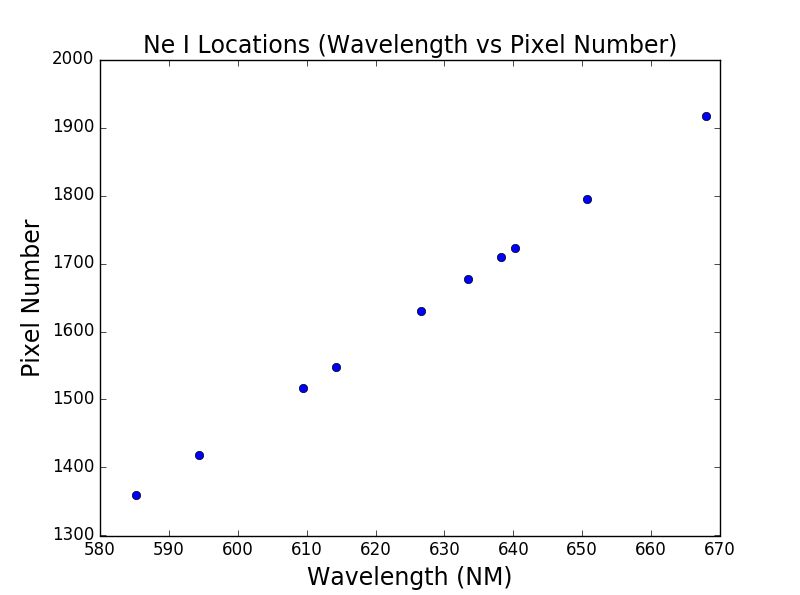
\includegraphics[width=.55\linewidth]{Ne1loc.png}
\end{subfigure}\par\medskip
\newline
\begin{flushleft}
Figure 5: Graphs of points plotted by comparing the centroid location of Hg I and Ne I emission lines. As expected, these points yield a linear behavior. 
\end{flushleft}

Although Figure 5 appears to be perfectly linear, there are still errors. We can measure these errors by fitting a line using the method of linear least squares and calculate the standard deviation between each points and the fit line:  

\begin{subfigure}{\linewidth}\hspace*{-1.3cm}
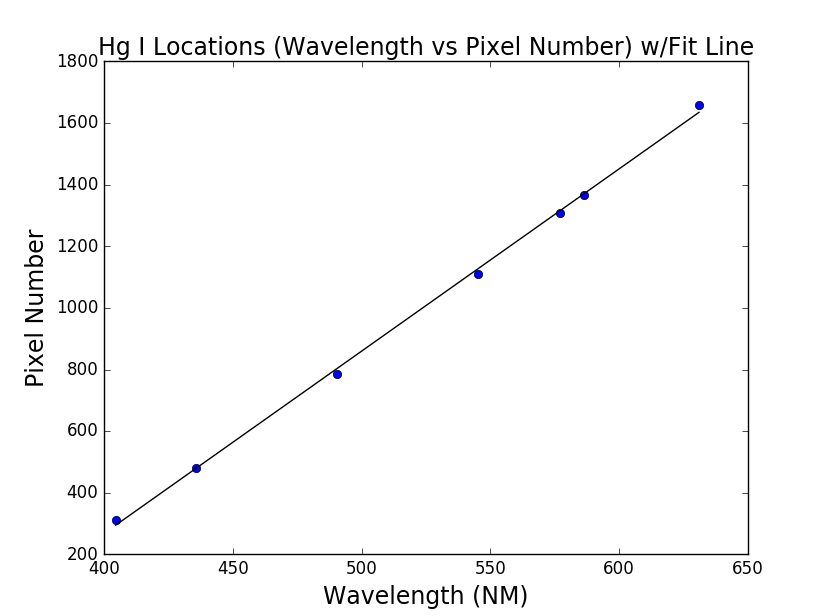
\includegraphics[width=.55\linewidth]{Hg1locline.png}
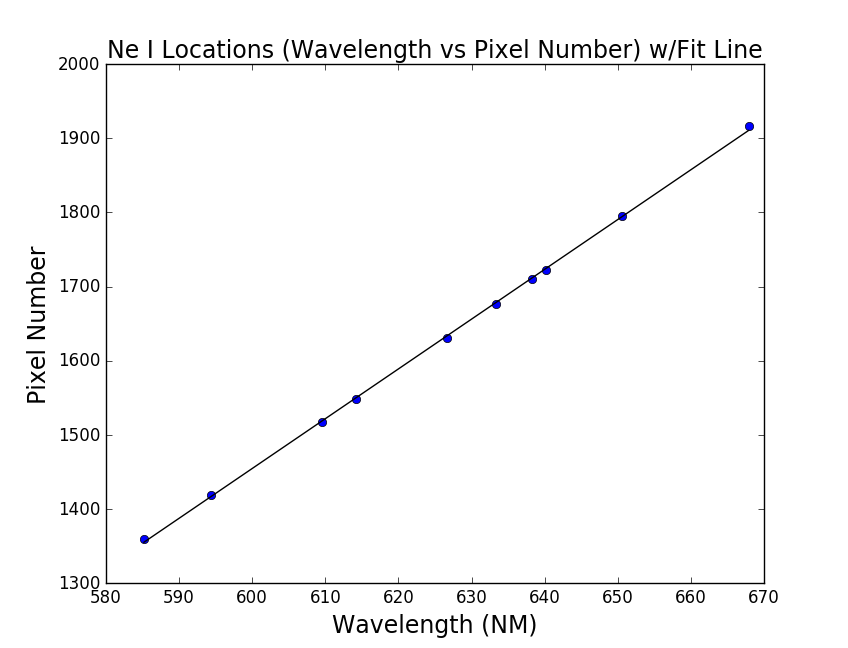
\includegraphics[width=.54\linewidth]{Ne1locline.png}
\end{subfigure}\par\medskip
\newline
\begin{flushleft}
Figure 6: Same graphs as Figure 5 but with fitted lines that showed imperfect linear behaviors between both Hg I and Ne I points. 
\end{flushleft}
Least squares fitted lines in Figure 6 can be expressed with the following equation: \[y = mx + c\] where m is the slope and c is the y-intercept. The Hg I line has the true value of m = 5.91908592 and c = -2099.97625. The Ne I line has the true value of m = 6.71314669 and c = -2573.23209. 

\section{Standard Deviations} \label{Std}
We can determine the error propagation by calculating the standard deviation of the slope and y-intercept for both Hg I and Ne I lines. First, we need to calculate the variance $\sigma$ of the slope and y-intercept. We can then calculate the standard deviation by square rooting the variance $\sqrt{\sigma}$. The variance of the slope for the Hg I line is 0.01235190 and the variance for the y-intercept is 3469.308093. The variance of the slope for the Ne I line is 0.00233550 and the variance for the y-intercept is 916.6730844. We can now take the square root of the variance to find the standard deviation. The standard deviation of slope for Ng I is 0.11113912 and 58.9008327 for the y-intercept. The standard deviation of slope for Ne I is 0.04832699 and 30.2766095 for the y-intercept. These results can be plotted onto a table shown as below:
\newline

\hspace*{-1cm}\begin{tabular}{ |p{1cm}||p{2cm}|p{2.3cm}|p{2.3cm}|p{2.3cm}|p{2cm}|p{2cm}| }
 \hline
 \multicolumn{7}{|c|}{Standard Deviation of the Fitted Ng I and Ne I Lines} \\
 \hline
 & Slope& y-intercept & Var of Slope & Var of y-int & Std of Slope & Std of y-int\\
 \hline
 Ng I & 5.91908592  & $-2099.97625$ & 0.01235190 & 3469.308093 & 0.11113912 & 58.9008327\\
 \hline
 Ne I & 6.71314669  & $-2573.23209$  & 0.00233550 & 916.6730844 & 0.04832699 & 30.2766095\\
 
 \hline
\end{tabular}
\newline
\begin{flushleft}
Table 1: The slope and y-intercept of fitted lines for Ng I and Ne I with the variances and their standard deviations.
\end{flushleft}

According to Table 1, the fitted line for Ng I has the average slope error of 0.11113912 and the fitted line for Ne I has the average slope error of 0.04832699. We now want to combine the Ng I and Ne I plots and test the linear least squares method's reliability. By appending the Ne I centroids into the Ng I plot we can get a graph that carries all the centroids from Ng I and Ne I. 
\newline
\centerline{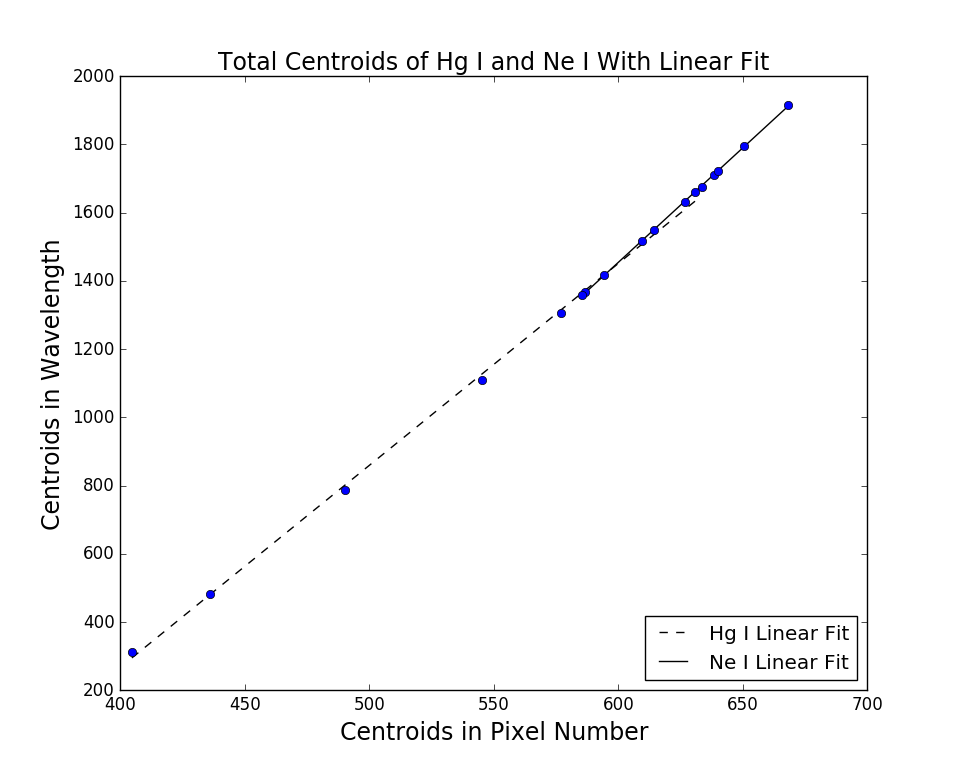
\includegraphics[scale = .4]{combcents.png}}
\begin{flushleft}
Figure 7: Combined centroid plot of Ng I and Ne I with their respective linear fit lines. The dash line represent the Hg I centroid linear fit and the darken line represent the Ne I centroid linear fit.
\end{flushleft}

In Figure 7, we can clearly see that the linear least squares method failed to create a best fit line for the combined centroid graph of Hg I and Ne I. This non-parallel relation between Hg I and Ne I lines showed that the linear least squares method don't work well with higher degree polynomials. We can create a better polynomial fit for Figure 7 by using a quadratic fit with second degree polynomial: 
\newline
\centerline{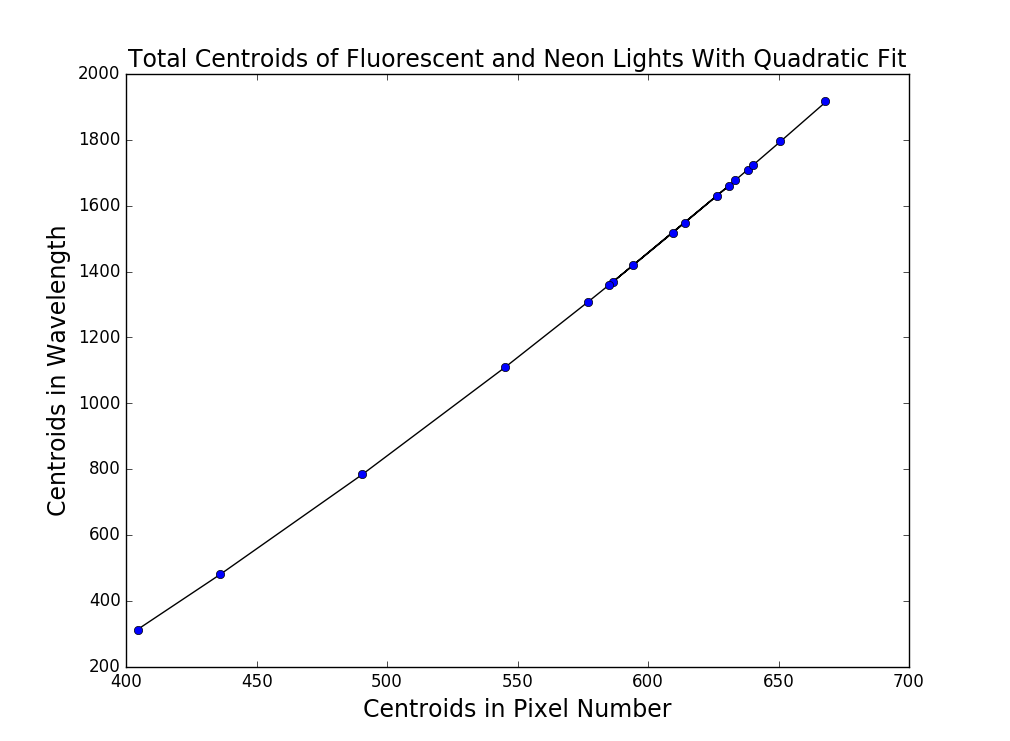
\includegraphics[scale = .38]{comcents2.png}}

\begin{flushleft}
Figure 8: Same as Figure 7 but with a quadratic fit line. We can see that the quadratic line fits better than the linear least squares line.
\end{flushleft}

\section{Read Noise \& Gain of the CCD Photon Detector} \label{CCD}

After the wavelength calibration, we can now measure the read noise and gain of the CCD detector.
By using the equation

\[\sigma^2_{ADU} = \frac{g \times e}{C} \times (ADU - ADU_o) + \sigma^2_{o}\]

where  $\sigma^2_{ADU}$ is the variance, $\frac{g \times e}{C}$ is the gain and $\sigma^2_{o}$ is the read noise. The resulted graph should have a linear behavior since it can be represented wth y = mx + c where the gain is the slope m and the read noise is the y-intercept c. The constant e is the charge of a single electron, g is the voltage of a single pulse generated by the CCD, C is the capacitance and $(ADU - ADU_o)$ is the mean bias subtracted signal which in our case, the combined mean wavelength of 30 sets of neon spectra: 

\centerline{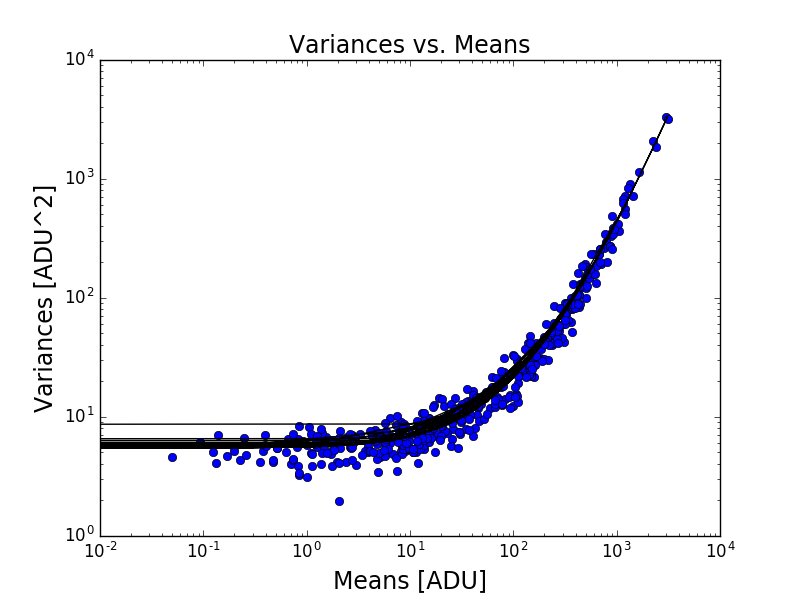
\includegraphics[scale = .45]{varmean.png}}
\newline
\begin{flushleft}
Figure 9: The variance versus the wavelength means from 30 sets of neon light spectra.
\end{flushleft}
We can now find the gain and read noise by determining the slope and y-intercept from the linear line in Figure 9. We can also find the variance and standard deviation of the gain and read noise using the method from an earlier section. The standard deviation of slope is the average error of each points from the linear line. The calculated value for gain is 0.6307846 and the read noise is 5.4503907:
\newline

\hspace*{-1.5cm}\begin{tabular}{ |p{1.6cm}||p{2cm}|p{2cm}|p{2cm}|p{2.4cm}|p{2.3cm}|p{2cm}| }
 \hline
 \multicolumn{7}{|c|}{Gain and Read Noise of the CCD and their Respective Errors} \\
 \hline
 & Gain& Read Noise & Var of Gain & Var of Noise & Error of Gain & Error of Noise\\
 \hline
 Figure 9 &  0.6307846 & 5.4503907 & $4.9008e{-5}$ & $9.928945e{-06}$ & $7.0005e{-3}$ & 0.0031510\\
 
 \hline
\end{tabular}
\newline
\begin{flushleft}
Table 2: The measured gain and read noise with respective variances and standard deviations.
\end{flushleft}

\section{Discussion}\label{Dis}
The reason behind why the Ocean Optics USB 2000 Spectrometer produces a "bias" intensity in all the graphs in Figure 1 is very vague to me. It might be caused by the photoelectric effect and small amount of photons are creating the noises. Even with the slit on the spectrometer is blocked, some photons can still reach inside the sensor. These small amount of photons could be the reason behind the noise with roughly 120 counts. This phenomenon can be observed on Figure 2, it the bias spectra. The bias spectra could be a design by Ocean Optic to avoid noises to reach to the negative counts if it maintain its average intensity around 0 count. We don't want negative data because it would make things very confusing. Another strange pattern is the absence of points near zero variance in Figure 9. This look very similar to the bias spectra but the reason for its origin is unknown to me.

\section{Conclusion}\label{Conc}
In this experiment my group have examined various light sources like Incandescent lamp, fluorescent strip light, color filters, neon gas discharge lamp, and sunlight by using the Ocean Optics USB 2000 Spectrometer. In Figure 1, each sources produce an unique set of spectra and we noticed each data have elevated overall intensity of roughly 120 counts. These intensity elevations were caused by the inherent property of the spectrometer to prevent the output of negative intensity. We eliminated that tiny intensity elevation by subtracting the Hg I and Ne I plots with the bias spectra collected by recording darkness with the spectrometer. By subtracting out the bias spectra we can then use the Hg I and Ne I spectra to obtain our centroids, that is the true location of each element's emission lines.

Once we have our centroids we can calibrate our wavelength by mapping the centroid positions of Hg I and Ne I in wavelength and pixel number and Figure 5 is our result. We then used the least squares method to fit a linear line to Figure 5 and get Figure 6. Once we have the fit lines for the centroids we can calculate the standard deviations for its slope and y-intercept. By knowing the standard deviation of the fit line we can check the spread or error of each centroid points for Hg I and Ne I. We then combine the total centroid points from Hg I and Ne I and create Figure 7 that showed an non-linear relationship between the Hg I and Ne I line. This shows that the least squares method does not work well with higher degrees of polynomials. We used a quadratic fit line to fit Figure 7 and get Figure 8.

Once we finish our wavelength calibration we can now measure the gain, read noise and saturation level of the CCD Photon Detector. By examining the spectra generated by SpectraSuite we observed a saturation level of 4096 counts by bringing the spectrometer close to a light source to create higher intensity. For the gain and read noise of the CCD Photon Detector we can use the variances and the means of each wavelength value from 30 sets of neon data to create a plot. By plotting the variances and the means we get Figure 9. The calculated gain of the CCD Photon Detector from Figure 9 is 0.6307846 and 5.4503907 for the read noise. We also found the error of the gain to be 0.007 and 0.003 for the read noise.

\begin{thebibliography}{9}

\bibitem{Graham} Graham, J. R. (2015). The Ocean Optics USB 2000 Spectrometer.\\

\\\texttt{https://drive.google.com/file/d/0B40Ynk22SiBpbXRnRlJRTHFtdzQ/view}

\bibitem{Graham} Graham, J. R. (2017). Finding the centroid: \big \langle x\big \rangle.\\

\\\texttt{https://drive.google.com/file/d/0B40Ynk22SiBpOW43MzFNRVNndTA/view}

\bibitem{Graham} Graham, J. R. (2017). Conventional Linear Least-Squares Fitting.\\

\\\texttt{https://drive.google.com/file/d/0B40Ynk22SiBpSU1DN2dPN3pzNXc/view}

\bibitem{Graham} Graham, J. R. (2017). A CCD Noise Model.\\

\\\texttt{https://drive.google.com/file/d/0B40Ynk22SiBpcEVwU25IcHF0R1E/view}
\end{thebibliography}


\end{document}
